\begin{minipage}{0.75\linewidth}
\begin{figure}[h]
    \centering
    \begin{adjustbox}{max width=1.0\linewidth, keepaspectratio}
        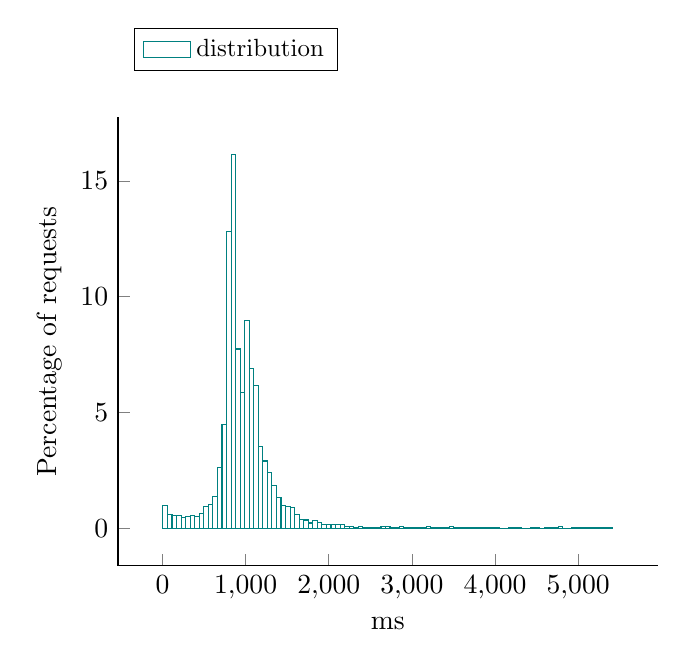
\begin{tikzpicture}
            \begin{axis}[ylabel = Percentage of requests, 
xlabel = ms, 
legend style = {nodes={scale=0.9, transform shape}, at={(0.03,1.2)}, anchor=north west, draw=black, fill=white, align=left, legend columns=3},
area style, mark size = 0pt,
 cycle list name = exotic,
  axis lines* = left]
		\addplot +[ybar interval] coordinates {
			 (5, 0.99612)
			 (59.64, 0.608158)
			 (114.28, 0.566216)
			 (168.92, 0.534759)
			 (223.56, 0.461361)
			 (278.2, 0.492817)
			 (332.84, 0.55573)
			 (387.48, 0.524274)
			 (442.12, 0.629129)
			 (496.76, 0.943693)
			 (551.4, 1.03806)
			 (606.04, 1.3736)
			 (660.68, 2.62137)
			 (715.32, 4.46681)
			 (769.96, 12.8237)
			 (824.6, 16.1267)
			 (879.24, 7.73828)
			 (933.88, 5.87187)
			 (988.52, 8.97557)
			 (1043.16, 6.89944)
			 (1097.8, 6.17595)
			 (1152.44, 3.53361)
			 (1207.08, 2.90448)
			 (1261.72, 2.39069)
			 (1316.36, 1.84544)
			 (1371, 1.33166)
			 (1425.64, 0.99612)
			 (1480.28, 0.922722)
			 (1534.92, 0.912237)
			 (1589.56, 0.608158)
			 (1644.2, 0.398448)
			 (1698.84, 0.356506)
			 (1753.48, 0.230681)
			 (1808.12, 0.32505)
			 (1862.76, 0.262137)
			 (1917.4, 0.178253)
			 (1972.04, 0.157282)
			 (2026.68, 0.146797)
			 (2081.32, 0.146797)
			 (2135.96, 0.178253)
			 (2190.6, 0.0629129)
			 (2245.24, 0.0733983)
			 (2299.88, 0.0524274)
			 (2354.52, 0.0629129)
			 (2409.16, 0.0314564)
			 (2463.8, 0.0419419)
			 (2518.44, 0.020971)
			 (2573.08, 0.0104855)
			 (2627.72, 0.0733983)
			 (2682.36, 0.0629129)
			 (2737, 0.0104855)
			 (2791.64, 0.0524274)
			 (2846.28, 0.0629129)
			 (2900.92, 0.0419419)
			 (2955.56, 0.0524274)
			 (3010.2, 0.0419419)
			 (3064.84, 0.0104855)
			 (3119.48, 0.0104855)
			 (3174.12, 0.0629129)
			 (3228.76, 0.020971)
			 (3283.4, 0.0419419)
			 (3338.04, 0.0104855)
			 (3392.68, 0.0419419)
			 (3447.32, 0.0838838)
			 (3501.96, 0.0104855)
			 (3556.6, 0.0314564)
			 (3611.24, 0.0419419)
			 (3665.88, 0.020971)
			 (3720.52, 0.0104855)
			 (3775.16, 0.020971)
			 (3829.8, 0.020971)
			 (3884.44, 0.0524274)
			 (3939.08, 0.0104855)
			 (3993.72, 0.020971)
			 (4048.36, 0)
			 (4103, 0)
			 (4157.64, 0.0419419)
			 (4212.28, 0.020971)
			 (4266.92, 0.0419419)
			 (4321.56, 0)
			 (4376.2, 0)
			 (4430.84, 0.0104855)
			 (4485.48, 0.0314564)
			 (4540.12, 0)
			 (4594.76, 0.0104855)
			 (4649.4, 0.0419419)
			 (4704.04, 0.0104855)
			 (4758.68, 0.0733983)
			 (4813.32, 0)
			 (4867.96, 0)
			 (4922.6, 0.020971)
			 (4977.24, 0.020971)
			 (5031.88, 0.020971)
			 (5086.52, 0.0314564)
			 (5141.16, 0.020971)
			 (5195.8, 0.0104855)
			 (5250.44, 0.0104855)
			 (5305.08, 0.020971)
			 (5359.72, 0.0104855)
			 (5414.36, 0.0104855)
		};
\addlegendentry{distribution};
           \end{axis}
      \end{tikzpicture}
  \end{adjustbox}
  \caption{Response time distribution - req = ReadUser-0}
\end{figure}
\end{minipage}\hfill\begin{minipage}{0.18\linewidth}
\begin{table}[h]
\begin{tabular}{|cc|}
\hline
\textbf{} & \textbf{ms}\\ \hline
 \Xhline{0.005\arrayrulewidth}
min & 5\\
 \Xhline{0.005\arrayrulewidth}
max & 5469\\
 \Xhline{0.005\arrayrulewidth}
mean & 993\\
 \Xhline{0.005\arrayrulewidth}
std & 463\\
\hline
\hline
 \Xhline{0.005\arrayrulewidth}
25th & 814\\
 \Xhline{0.005\arrayrulewidth}
50th & 911\\
 \Xhline{0.005\arrayrulewidth}
75th & 1104\\
 \Xhline{0.005\arrayrulewidth}
80th & 1148\\
 \Xhline{0.005\arrayrulewidth}
85th & 1228\\
 \Xhline{0.005\arrayrulewidth}
90th & 1338\\
 \Xhline{0.005\arrayrulewidth}
95th & 1573\\
 \Xhline{0.005\arrayrulewidth}
99th & 3064\\
\hline
\end{tabular}
\caption{Response time}
\end{table}
\end{minipage}\hfill